%%%%%%%%%%%%%%%%%%%%%%%%%%%%%%%%%%%%%%%%%%%%%%%%%%%%%%%%%%%%%%%%%%%%%%%%%%%%%%%%
% Template for USENIX papers.
%
% History:
%
% - TEMPLATE for Usenix papers, specifically to meet requirements of
%   USENIX '05. originally a template for producing IEEE-format
%   articles using LaTeX. written by Matthew Ward, CS Department,
%   Worcester Polytechnic Institute. adapted by David Beazley for his
%   excellent SWIG paper in Proceedings, Tcl 96. turned into a
%   smartass generic template by De Clarke, with thanks to both the
%   above pioneers. Use at your own risk. Complaints to /dev/null.
%   Make it two column with no page numbering, default is 10 point.
%
% - Munged by Fred Douglis <douglis@research.att.com> 10/97 to
%   separate the .sty file from the LaTeX source template, so that
%   people can more easily include the .sty file into an existing
%   document. Also changed to more closely follow the style guidelines
%   as represented by the Word sample file.
%
% - Note that since 2010, USENIX does not require endnotes. If you
%   want foot of page notes, don't include the endnotes package in the
%   usepackage command, below.
% - This version uses the latex2e styles, not the very ancient 2.09
%   stuff.
%
% - Updated July 2018: Text block size changed from 6.5" to 7"
%
% - Updated Dec 2018 for ATC'19:
%
%   * Revised text to pass HotCRP's auto-formatting check, with
%     hotcrp.settings.submission_form.body_font_size=10pt, and
%     hotcrp.settings.submission_form.line_height=12pt
%
%   * Switched from \endnote-s to \footnote-s to match Usenix's policy.
%
%   * \section* => \begin{abstract} ... \end{abstract}
%
%   * Make template self-contained in terms of bibtex entires, to allow
%     this file to be compiled. (And changing refs style to 'plain'.)
%
%   * Make template self-contained in terms of figures, to
%     allow this file to be compiled. 
%
%   * Added packages for hyperref, embedding fonts, and improving
%     appearance.
%   
%   * Removed outdated text.
%
%%%%%%%%%%%%%%%%%%%%%%%%%%%%%%%%%%%%%%%%%%%%%%%%%%%%%%%%%%%%%%%%%%%%%%%%%%%%%%%%

\documentclass[letterpaper,twocolumn,10pt]{article}
\usepackage{usenix-2020-09}

% to be able to draw some self-contained figs
\usepackage{tikz}
\usepackage{amsmath}

% inlined bib file
\usepackage{filecontents}

%-------------------------------------------------------------------------------
\begin{filecontents}{\jobname.bib}
%-------------------------------------------------------------------------------
@misc{gu20ropriscv,
    title={Return-Oriented Programming in RISC-V}, 
    author={Gu, Garrett and Shacham, Hovav},
    year={2020},
    eprint={2007.14995},
    archivePrefix={arXiv},
    primaryClass={cs.CR},
}
@inproceedings{bletsch11jopx86,
    author = {Bletsch, Tyler and Jiang, Xuxian and Freeh, Vince W. and Liang, Zhenkai},
    title = {Jump-Oriented Programming: A New Class of Code-Reuse Attack},
    year = {2011},
    isbn = {9781450305648},
    publisher = {Association for Computing Machinery},
    address = {New York, NY, USA},
    url = {https://doi.org/10.1145/1966913.1966919},
    doi = {10.1145/1966913.1966919},
    abstract = {Return-oriented programming is an effective code-reuse attack in which short code sequences ending in a ret instruction are found within existing binaries and executed in arbitrary order by taking control of the stack. This allows for Turing-complete behavior in the target program without the need for injecting attack code, thus significantly negating current code injection defense efforts (e.g., W⊕X). On the other hand, its inherent characteristics, such as the reliance on the stack and the consecutive execution of return-oriented gadgets, have prompted a variety of defenses to detect or prevent it from happening.In this paper, we introduce a new class of code-reuse attack, called jump-oriented programming. This new attack eliminates the reliance on the stack and ret instructions (including ret-like instructions such as pop+jmp) seen in return-oriented programming without sacrificing expressive power. This attack still builds and chains functional gadgets, each performing certain primitive operations, except these gadgets end in an indirect branch rather than ret. Without the convenience of using ret to unify them, the attack relies on a dispatcher gadget to dispatch and execute the functional gadgets. We have successfully identified the availability of these jump-oriented gadgets in the GNU libc library. Our experience with an example shellcode attack demonstrates the practicality and effectiveness of this technique.},
    booktitle = {Proceedings of the 6th ACM Symposium on Information, Computer and Communications Security},
    pages = {30–40},
    numpages = {11},
    location = {Hong Kong, China},
    series = {ASIACCS '11}
}
@inproceedings{shacham07ropx86,
    author = {Shacham, Hovav},
    title = {The Geometry of Innocent Flesh on the Bone: Return-into-Libc without Function Calls (on the X86)},
    year = {2007},
    isbn = {9781595937032},
    publisher = {Association for Computing Machinery},
    address = {New York, NY, USA},
    url = {https://doi.org/10.1145/1315245.1315313},
    doi = {10.1145/1315245.1315313},
    abstract = {We present new techniques that allow a return-into-libc attack to be mounted on x86 executables that calls no functions at all. Our attack combines a large number of short instruction sequences to build gadgets that allow arbitrary computation. We show how to discover such instruction sequences by means of static analysis. We make use, in an essential way, of the properties of the x86 instruction set.},
    booktitle = {Proceedings of the 14th ACM Conference on Computer and Communications Security},
    pages = {552–561},
    numpages = {10},
    keywords = {return-into-libc, instruction set, turing completeness},
    location = {Alexandria, Virginia, USA},
    series = {CCS '07}
}
@inproceedings{patterson98risc,
    title={RISC I: A reduced instruction set VLSI computer},
    author={Patterson, David A and Sequin, Carlo H},
    booktitle={25 years of the international symposia on Computer architecture (selected papers)},
    pages={216--230},
    year={1998}
}

\end{filecontents}

%-------------------------------------------------------------------------------
\begin{document}
%-------------------------------------------------------------------------------

%don't want date printed
\date{}

% make title bold and 14 pt font (Latex default is non-bold, 16 pt)
\title{\Large \bf JOP in RISC-V:\\
  (working title)}

%for single author (just remove % characters)
\author{
{\rm Daniel Starikov}\\
Univeristy of Washington
\and
{\rm Keanu Vestil}\\
University of Washington
% copy the following lines to add more authors
% \and
% {\rm Name}\\
%Name Institution
} % end author

\maketitle

%-------------------------------------------------------------------------------
\begin{abstract}
%-------------------------------------------------------------------------------
Your abstract text goes here. Just a few facts. Whet our appetites.
Not more than 200 words, if possible, and preferably closer to 150.
\end{abstract}


%-------------------------------------------------------------------------------
\section{Introduction}
%-------------------------------------------------------------------------------

RISC-V is a free and open instruction set architecture (ISA) introduced by UC
Berkeley in 2010. Although it was initially designed for research and education
purposes, it is being increasingly used in commercial settings. RISC-V is a
based on the reduced instruction set computer (RISC) paradigm. This aims to
improve a machine's throughput by simplifying instructions and addressing modes,
thus reducing the cycles needed per instruction and reducing the time per cycle~\cite{patterson98risc}.

[paragraph about code reuse attacks]

[paragraph about ROP and JOP]

[paragraph about]

%-------------------------------------------------------------------------------
\section{Footnotes, Verbatim, and Citations Examples}
%-------------------------------------------------------------------------------

Footnotes should be places after punctuation characters, without any
spaces between said characters and footnotes, like so.%
\footnote{Remember that USENIX format stopped using endnotes and is
  now using regular footnotes.} And some embedded literal code may
look as follows.

\begin{verbatim}
int main(int argc, char *argv[]) 
{
    return 0;
}
\end{verbatim}

This is an example citation of Gu and Shacham~\cite{gu20ropriscv}. This is an
example of citing two papers at once, which both discuss x86-based code reuse
attacks~\cite{shacham07ropx86,bletsch11jopx86}.

The tilde character (\~{}) in the tex source means a non-breaking
space. This way, your reference will always be attached to the word
that preceded it, instead of going to the next line.

And the 'cite' package sorts your citations by their numerical order
of the corresponding references at the end of the paper.

It'd be nice and thoughtful of you to include a suitable link in each
and every bibtex entry that you use in your submission, to allow
reviewers (and other readers) to easily get to the cited work.

Now we're going take a look at Section~\ref{sec:figs}, but not before
observing that refs to sections and citations and such are colored and
clickable in the PDF because of the packages we've included.

%-------------------------------------------------------------------------------
\section{Floating Figures and Lists}
\label{sec:figs}
%-------------------------------------------------------------------------------


%---------------------------
\begin{figure}
\begin{center}
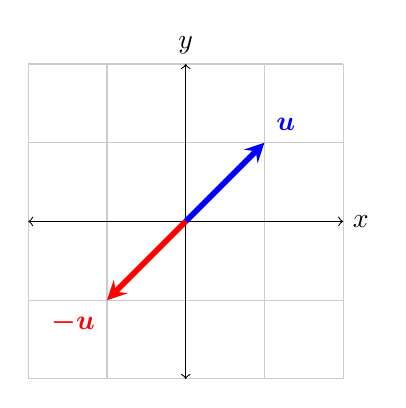
\begin{tikzpicture}
  \draw[thin,gray!40] (-2,-2) grid (2,2);
  \draw[<->] (-2,0)--(2,0) node[right]{$x$};
  \draw[<->] (0,-2)--(0,2) node[above]{$y$};
  \draw[line width=2pt,blue,-stealth](0,0)--(1,1)
        node[anchor=south west]{$\boldsymbol{u}$};
  \draw[line width=2pt,red,-stealth](0,0)--(-1,-1)
        node[anchor=north east]{$\boldsymbol{-u}$};
\end{tikzpicture}
\end{center}
\caption{\label{fig:vectors} Text size inside figure should be as big as
  caption's text. Text size inside figure should be as big as
  caption's text. Text size inside figure should be as big as
  caption's text. Text size inside figure should be as big as
  caption's text. Text size inside figure should be as big as
  caption's text. }
\end{figure}
%% %---------------------------


Here's a typical reference to a floating figure:
Figure~\ref{fig:vectors}. Floats should usually be placed where latex
wants then. Figure\ref{fig:vectors} is centered, and has a caption
that instructs you to make sure that the size of the text within the
figures that you use is as big as (or bigger than) the size of the
text in the caption of the figures. Please do. Really.

In our case, we've explicitly drawn the figure inlined in latex, to
allow this tex file to cleanly compile. But usually, your figures will
reside in some file.pdf, and you'd include them in your document
with, say, \textbackslash{}includegraphics.

Lists are sometimes quite handy. If you want to itemize things, feel
free:

\begin{description}
  
\item[fread] a function that reads from a \texttt{stream} into the
  array \texttt{ptr} at most \texttt{nobj} objects of size
  \texttt{size}, returning returns the number of objects read.

\item[Fred] a person's name, e.g., there once was a dude named Fred
  who separated usenix.sty from this file to allow for easy
  inclusion.
\end{description}

\noindent
The noindent at the start of this paragraph in its tex version makes
it clear that it's a continuation of the preceding paragraph, as
opposed to a new paragraph in its own right.


\subsection{LaTeX-ing Your TeX File}
%-----------------------------------

People often use \texttt{pdflatex} these days for creating pdf-s from
tex files via the shell. And \texttt{bibtex}, of course. Works for us.

%-------------------------------------------------------------------------------
\section*{Acknowledgments}
%-------------------------------------------------------------------------------

The USENIX latex style is old and very tired, which is why
there's no \textbackslash{}acks command for you to use when
acknowledging. Sorry.

%-------------------------------------------------------------------------------
\section*{Availability}
%-------------------------------------------------------------------------------

USENIX program committees give extra points to submissions that are
backed by artifacts that are publicly available. If you made your code
or data available, it's worth mentioning this fact in a dedicated
section.

%-------------------------------------------------------------------------------
\bibliographystyle{plain}
\bibliography{\jobname}

%%%%%%%%%%%%%%%%%%%%%%%%%%%%%%%%%%%%%%%%%%%%%%%%%%%%%%%%%%%%%%%%%%%%%%%%%%%%%%%%
\end{document}
%%%%%%%%%%%%%%%%%%%%%%%%%%%%%%%%%%%%%%%%%%%%%%%%%%%%%%%%%%%%%%%%%%%%%%%%%%%%%%%%

%%  LocalWords:  endnotes includegraphics fread ptr nobj noindent
%%  LocalWords:  pdflatex acks
